\def\notedate{2023.01.10}
\def\currentauthor{Журавлев Н.В. (РК6-72Б)}
\notestatement{rndhpcedt}{Рассмотрение алгоритмов для поиска циклов в графе из книги Евстигнеева и Касьянова Графы в программировании}
Из книги Евстигнеева и Касьянова "Графы в программировании" были рассмотрены и проанализированы следующие алгоритмы\cite{eg-graph}:

Рекурсивный алгоритм обхода графа в глубину (Рисунок \ref{fig:rec}) не желательно для использования, т.к. имеется рекурсия, что может плохо сказать при выполнении поиска.

\begin{figure}[h!]
    \centering
    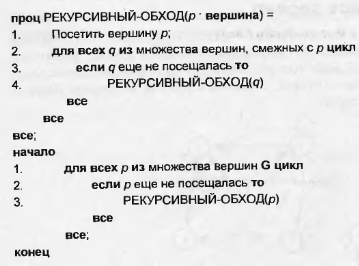
\includegraphics[width=0.4\linewidth]{ResearchNotes/rndhpc_int_edt_2023_01_10/rec.png}
    \caption{Рекурсивный алгоритм обхода графа в глубину}
    \label{fig:rec}
\end{figure}

Общий алгоритм обхода графа с запоминанием дуг (Рисунок \ref{fig:save_arc}) и общий алгоритм обхода графа с запоминанием вершин (Рисунок \ref{fig:save_eages}) имеют одинаковые характеристики, которые подходят под заданный граф.

\begin{figure}[h!]
    \centering
    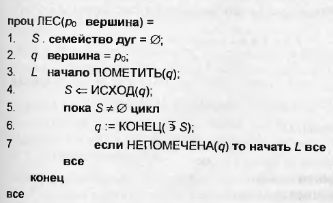
\includegraphics[width=0.4\linewidth]{ResearchNotes/rndhpc_int_edt_2023_01_10/save_arc.png}
    \caption{Общий алгоритм обхода графа с запоминанием дуг}
    \label{fig:save_arc}
\end{figure}

\begin{figure}[h!]
    \centering
    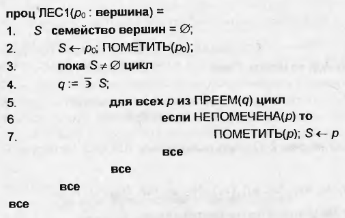
\includegraphics[width=0.4\linewidth]{ResearchNotes/rndhpc_int_edt_2023_01_10/save_eages.png}
    \caption{Общий алгоритм обхода графа с запоминанием вершин}
    \label{fig:save_eages}
\end{figure}

Алгоритм обхода графа в ширину с использованием внешней очереди (Рисунок \ref{fig:outer_queue}) и алгоритм обхода графа в ширину с использованием внутренней очереди (Рисунок \ref{fig:internal _queue}). Оба алгоритма не подходят, так как имеют большую временную сложность, а именно O$(k + t)$, где k и t - количество дуг и вершин графа, по сравнению с общим алгоритмом обхода графа с запоминанием вершин, который имеет сложность O$(t)$, где t - количество дуг.

\begin{figure}[h!]
    \centering
    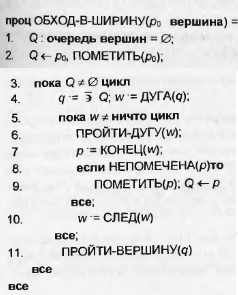
\includegraphics[width=0.4\linewidth]{ResearchNotes/rndhpc_int_edt_2023_01_10/outer_queue.png}
    \caption{Алгоритм обхода графа в ширину с использованием внешней очереди}
    \label{fig:outer_queue}
\end{figure}

\begin{figure}[h!]
    \centering
    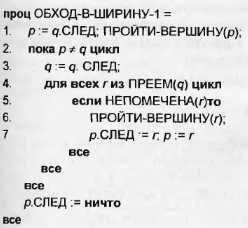
\includegraphics[width=0.4\linewidth]{ResearchNotes/rndhpc_int_edt_2023_01_10/internal_queue.png}
    \caption{Алгоритм обхода графа в ширину с использованием внутренней очереди}
    \label{fig:internal _queue}
\end{figure}

Алгоритм обхода графа в глубину без использование дополнительной памяти, представленный в (Рисунок \ref{fig:without_memory}) не подходит, так как его работы необходим один приёмник из начальной вершины.

\begin{figure}[h!]
    \centering
    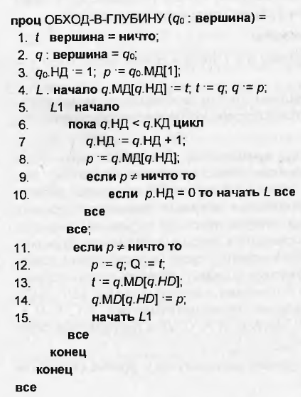
\includegraphics[width=0.4\linewidth]{ResearchNotes/rndhpc_int_edt_2023_01_10/without_memory.png}
    \caption{Алгоритм обхода графа в глубину без использование дополнительной памяти}
    \label{fig:without_memory}
\end{figure}

\noteattributes{}